\documentclass[twoside]{book}

% Packages required by doxygen
\usepackage{calc}
\usepackage{doxygen}
\usepackage{graphicx}
\usepackage[utf8]{inputenc}
\usepackage{makeidx}
\usepackage{multicol}
\usepackage{multirow}
\usepackage{fixltx2e}
\PassOptionsToPackage{warn}{textcomp}
\usepackage{textcomp}
\usepackage[nointegrals]{wasysym}
\usepackage[table]{xcolor}

% Font selection
\usepackage[T1]{fontenc}
\usepackage{mathptmx}
\usepackage[scaled=.90]{helvet}
\usepackage{courier}
\usepackage{amssymb}
\usepackage{sectsty}
\renewcommand{\familydefault}{\sfdefault}
\allsectionsfont{%
  \fontseries{bc}\selectfont%
  \color{darkgray}%
}
\renewcommand{\DoxyLabelFont}{%
  \fontseries{bc}\selectfont%
  \color{darkgray}%
}
\newcommand{\+}{\discretionary{\mbox{\scriptsize$\hookleftarrow$}}{}{}}

% Page & text layout
\usepackage{geometry}
\geometry{%
  a4paper,%
  top=2.5cm,%
  bottom=2.5cm,%
  left=2.5cm,%
  right=2.5cm%
}
\tolerance=750
\hfuzz=15pt
\hbadness=750
\setlength{\emergencystretch}{15pt}
\setlength{\parindent}{0cm}
\setlength{\parskip}{0.2cm}
\makeatletter
\renewcommand{\paragraph}{%
  \@startsection{paragraph}{4}{0ex}{-1.0ex}{1.0ex}{%
    \normalfont\normalsize\bfseries\SS@parafont%
  }%
}
\renewcommand{\subparagraph}{%
  \@startsection{subparagraph}{5}{0ex}{-1.0ex}{1.0ex}{%
    \normalfont\normalsize\bfseries\SS@subparafont%
  }%
}
\makeatother

% Headers & footers
\usepackage{fancyhdr}
\pagestyle{fancyplain}
\fancyhead[LE]{\fancyplain{}{\bfseries\thepage}}
\fancyhead[CE]{\fancyplain{}{}}
\fancyhead[RE]{\fancyplain{}{\bfseries\leftmark}}
\fancyhead[LO]{\fancyplain{}{\bfseries\rightmark}}
\fancyhead[CO]{\fancyplain{}{}}
\fancyhead[RO]{\fancyplain{}{\bfseries\thepage}}
\fancyfoot[LE]{\fancyplain{}{}}
\fancyfoot[CE]{\fancyplain{}{}}
\fancyfoot[RE]{\fancyplain{}{\bfseries\scriptsize Generated on Mon Aug 4 2014 13\+:36\+:29 for Fast\+B\+S\+O\+N by Doxygen }}
\fancyfoot[LO]{\fancyplain{}{\bfseries\scriptsize Generated on Mon Aug 4 2014 13\+:36\+:29 for Fast\+B\+S\+O\+N by Doxygen }}
\fancyfoot[CO]{\fancyplain{}{}}
\fancyfoot[RO]{\fancyplain{}{}}
\renewcommand{\footrulewidth}{0.4pt}
\renewcommand{\chaptermark}[1]{%
  \markboth{#1}{}%
}
\renewcommand{\sectionmark}[1]{%
  \markright{\thesection\ #1}%
}

% Indices & bibliography
\usepackage{natbib}
\usepackage[titles]{tocloft}
\setcounter{tocdepth}{3}
\setcounter{secnumdepth}{5}
\makeindex

% Hyperlinks (required, but should be loaded last)
\usepackage{ifpdf}
\ifpdf
  \usepackage[pdftex,pagebackref=true]{hyperref}
\else
  \usepackage[ps2pdf,pagebackref=true]{hyperref}
\fi
\hypersetup{%
  colorlinks=true,%
  linkcolor=blue,%
  citecolor=blue,%
  unicode%
}

% Custom commands
\newcommand{\clearemptydoublepage}{%
  \newpage{\pagestyle{empty}\cleardoublepage}%
}


%===== C O N T E N T S =====

\begin{document}

% Titlepage & ToC
\hypersetup{pageanchor=false,
             bookmarks=true,
             bookmarksnumbered=true,
             pdfencoding=unicode
            }
\pagenumbering{roman}
\begin{titlepage}
\vspace*{7cm}
\begin{center}%
{\Large Fast\+B\+S\+O\+N }\\
\vspace*{1cm}
{\large Generated by Doxygen 1.8.7}\\
\vspace*{0.5cm}
{\small Mon Aug 4 2014 13:36:29}\\
\end{center}
\end{titlepage}
\clearemptydoublepage
\tableofcontents
\clearemptydoublepage
\pagenumbering{arabic}
\hypersetup{pageanchor=true}

%--- Begin generated contents ---
\chapter{Hierarchical Index}
\section{Class Hierarchy}
This inheritance list is sorted roughly, but not completely, alphabetically\+:\begin{DoxyCompactList}
\item \contentsline{section}{bson\+:\+:Document}{\pageref{classbson_1_1_document}}{}
\item \contentsline{section}{bson\+:\+:Element}{\pageref{classbson_1_1_element}}{}
\item exception\begin{DoxyCompactList}
\item \contentsline{section}{bson\+:\+:type\+\_\+error$<$ T $>$}{\pageref{classbson_1_1type__error}}{}
\item \contentsline{section}{bson\+:\+:type\+\_\+\+U\+N\+K\+N\+O\+W\+N}{\pageref{classbson_1_1type___u_n_k_n_o_w_n}}{}
\end{DoxyCompactList}
\end{DoxyCompactList}

\chapter{Class Index}
\section{Class List}
Here are the classes, structs, unions and interfaces with brief descriptions\+:\begin{DoxyCompactList}
\item\contentsline{section}{\hyperlink{classbson_1_1_document}{bson\+::\+Document} }{\pageref{classbson_1_1_document}}{}
\item\contentsline{section}{\hyperlink{classbson_1_1_element}{bson\+::\+Element} }{\pageref{classbson_1_1_element}}{}
\item\contentsline{section}{\hyperlink{classbson_1_1type__error}{bson\+::type\+\_\+error$<$ T $>$} }{\pageref{classbson_1_1type__error}}{}
\item\contentsline{section}{\hyperlink{classbson_1_1type___u_n_k_n_o_w_n}{bson\+::type\+\_\+\+U\+N\+K\+N\+O\+W\+N} }{\pageref{classbson_1_1type___u_n_k_n_o_w_n}}{}
\end{DoxyCompactList}

\chapter{File Index}
\section{File List}
Here is a list of all documented files with brief descriptions\+:\begin{DoxyCompactList}
\item\contentsline{section}{\hyperlink{document_8h}{document.\+h} \\*Definition of the B\+S\+O\+N Document class }{\pageref{document_8h}}{}
\item\contentsline{section}{\hyperlink{element_8h}{element.\+h} \\*Declaration of a B\+S\+O\+N element }{\pageref{element_8h}}{}
\item\contentsline{section}{\hyperlink{element_8hpp}{element.\+hpp} \\*Implementation of the B\+S\+O\+N element class }{\pageref{element_8hpp}}{}
\item\contentsline{section}{\hyperlink{typeinfo_8h}{typeinfo.\+h} \\*Enumeration to keep track of types for bson }{\pageref{typeinfo_8h}}{}
\end{DoxyCompactList}

\chapter{Class Documentation}
\hypertarget{classbson_1_1_document}{\section{bson\+:\+:Document Class Reference}
\label{classbson_1_1_document}\index{bson\+::\+Document@{bson\+::\+Document}}
}
\subsection*{Public Member Functions}
\begin{DoxyCompactItemize}
\item 
\hyperlink{classbson_1_1_document_ac2d96a9a7cc578ad769120bb1757a72d}{Document} (std\+::initializer\+\_\+list$<$ std\+::pair$<$ std\+::string, \hyperlink{classbson_1_1_element}{Element} $>$$>$ list)
\begin{DoxyCompactList}\small\item\em Initialization list constructor. \end{DoxyCompactList}\item 
const \hyperlink{classbson_1_1_element}{Element} \& \hyperlink{classbson_1_1_document_a37575739ba04bc0cdeab04828fcd6d7d}{operator\mbox{[}$\,$\mbox{]}} (const std\+::string \&index) const 
\begin{DoxyCompactList}\small\item\em accessor \end{DoxyCompactList}\item 
\hypertarget{classbson_1_1_document_a526ef4900d0842b9d2bf699dd32da7e4}{\hyperlink{classbson_1_1_element}{Element} \& {\bfseries operator\mbox{[}$\,$\mbox{]}} (const std\+::string \&index)}\label{classbson_1_1_document_a526ef4900d0842b9d2bf699dd32da7e4}

\item 
void \hyperlink{classbson_1_1_document_a1fea885e6efb76119b8e75dab2ed1ff2}{add} (const std\+::string name, const \hyperlink{classbson_1_1_element}{Element} \&data)
\begin{DoxyCompactList}\small\item\em element addition \end{DoxyCompactList}\item 
{\footnotesize template$<$class T $>$ }\\void \hyperlink{classbson_1_1_document_af4207bd81fead053e679cbbecaac294e}{add} (const std\+::string name, const T \&data, const Type\+Info ti=\+\_\+\+U\+N\+K\+N\+O\+W\+N)
\begin{DoxyCompactList}\small\item\em element addition \end{DoxyCompactList}\item 
void \hyperlink{classbson_1_1_document_a2dd4dee4cae8930d3f35acb6badf1c9b}{set} (const std\+::string name, const \hyperlink{classbson_1_1_element}{Element} \&data)
\begin{DoxyCompactList}\small\item\em element modification \end{DoxyCompactList}\item 
{\footnotesize template$<$class T $>$ }\\void \hyperlink{classbson_1_1_document_af8c1c129a0b8a21a1ab3a719e9677d0b}{set} (const std\+::string \&name, const T \&data, const Type\+Info ti=\+\_\+\+U\+N\+K\+N\+O\+W\+N)
\begin{DoxyCompactList}\small\item\em element modification \end{DoxyCompactList}\item 
auto \hyperlink{classbson_1_1_document_ae4387eb48d47787eed0a0c7d46214433}{begin} () -\/$>$ decltype(m\+\_\+data.\+begin())
\begin{DoxyCompactList}\small\item\em iterator functions \end{DoxyCompactList}\item 
\hypertarget{classbson_1_1_document_a261933f02ab97f8c3630a6bd978bf72b}{auto {\bfseries end} () -\/$>$ decltype(m\+\_\+data.\+end())}\label{classbson_1_1_document_a261933f02ab97f8c3630a6bd978bf72b}

\item 
\hypertarget{classbson_1_1_document_a8e77cea1e110d8e6c9f1eaec1e762e80}{auto {\bfseries rbegin} () -\/$>$ decltype(m\+\_\+data.\+rbegin())}\label{classbson_1_1_document_a8e77cea1e110d8e6c9f1eaec1e762e80}

\item 
\hypertarget{classbson_1_1_document_a3dbd675ec728ae5e5869f96e2e341b3d}{auto {\bfseries rend} () -\/$>$ decltype(m\+\_\+data.\+rend())}\label{classbson_1_1_document_a3dbd675ec728ae5e5869f96e2e341b3d}

\item 
\hypertarget{classbson_1_1_document_a981b86245cd36a13432e66c14329d585}{auto {\bfseries cbegin} () -\/$>$ decltype(m\+\_\+data.\+cbegin())}\label{classbson_1_1_document_a981b86245cd36a13432e66c14329d585}

\item 
\hypertarget{classbson_1_1_document_a1b3d3866623fd1953f5a70b337c2b18a}{auto {\bfseries cend} () -\/$>$ decltype(m\+\_\+data.\+cend())}\label{classbson_1_1_document_a1b3d3866623fd1953f5a70b337c2b18a}

\item 
\hypertarget{classbson_1_1_document_a050381182bf3f92ac472950cc62a14b4}{auto {\bfseries crbegin} () -\/$>$ decltype(m\+\_\+data.\+crbegin())}\label{classbson_1_1_document_a050381182bf3f92ac472950cc62a14b4}

\item 
\hypertarget{classbson_1_1_document_a1667c39ae48b51087452e34f6200ebe9}{auto {\bfseries crend} () -\/$>$ decltype(m\+\_\+data.\+crend())}\label{classbson_1_1_document_a1667c39ae48b51087452e34f6200ebe9}

\item 
std\+::set$<$ std\+::string $>$ \hyperlink{classbson_1_1_document_a4d0e6f7f9d1ba20e709ddc7e46bd00a0}{field\+\_\+names} () const 
\begin{DoxyCompactList}\small\item\em returns the set of field names \end{DoxyCompactList}\end{DoxyCompactItemize}
\subsection*{Friends}
\begin{DoxyCompactItemize}
\item 
\hypertarget{classbson_1_1_document_a016b821f88c7c0a2de1451c175cefbf9}{class {\bfseries Element}}\label{classbson_1_1_document_a016b821f88c7c0a2de1451c175cefbf9}

\item 
std\+::ostream \& \hyperlink{classbson_1_1_document_a66f02c1ef7b76d9bc4373b503585c6e9}{operator$<$$<$} (std\+::ostream \&o, const \hyperlink{classbson_1_1_document}{Document} \&d)
\begin{DoxyCompactList}\small\item\em insertion operator overloading \end{DoxyCompactList}\end{DoxyCompactItemize}


\subsection{Constructor \& Destructor Documentation}
\hypertarget{classbson_1_1_document_ac2d96a9a7cc578ad769120bb1757a72d}{\index{bson\+::\+Document@{bson\+::\+Document}!Document@{Document}}
\index{Document@{Document}!bson\+::\+Document@{bson\+::\+Document}}
\subsubsection[{Document}]{\setlength{\rightskip}{0pt plus 5cm}bson\+::\+Document\+::\+Document (
\begin{DoxyParamCaption}
\item[{std\+::initializer\+\_\+list$<$ std\+::pair$<$ std\+::string, {\bf Element} $>$$>$}]{list}
\end{DoxyParamCaption}
)\hspace{0.3cm}{\ttfamily [inline]}}}\label{classbson_1_1_document_ac2d96a9a7cc578ad769120bb1757a72d}


Initialization list constructor. 

\begin{DoxyPrecond}{Precondition}
None 
\end{DoxyPrecond}
\begin{DoxyPostcond}{Postcondition}
Constructs the dictionary using the init list of key/value pairs 
\end{DoxyPostcond}


\subsection{Member Function Documentation}
\hypertarget{classbson_1_1_document_a1fea885e6efb76119b8e75dab2ed1ff2}{\index{bson\+::\+Document@{bson\+::\+Document}!add@{add}}
\index{add@{add}!bson\+::\+Document@{bson\+::\+Document}}
\subsubsection[{add}]{\setlength{\rightskip}{0pt plus 5cm}void bson\+::\+Document\+::add (
\begin{DoxyParamCaption}
\item[{const std\+::string}]{name, }
\item[{const {\bf Element} \&}]{data}
\end{DoxyParamCaption}
)\hspace{0.3cm}{\ttfamily [inline]}}}\label{classbson_1_1_document_a1fea885e6efb76119b8e75dab2ed1ff2}


element addition 

\begin{DoxyPrecond}{Precondition}
None 
\end{DoxyPrecond}
\begin{DoxyPostcond}{Postcondition}
creates the element in the map. If name already exists in the document the value is overwritten 
\end{DoxyPostcond}
\hypertarget{classbson_1_1_document_af4207bd81fead053e679cbbecaac294e}{\index{bson\+::\+Document@{bson\+::\+Document}!add@{add}}
\index{add@{add}!bson\+::\+Document@{bson\+::\+Document}}
\subsubsection[{add}]{\setlength{\rightskip}{0pt plus 5cm}template$<$class T $>$ void bson\+::\+Document\+::add (
\begin{DoxyParamCaption}
\item[{const std\+::string}]{name, }
\item[{const T \&}]{data, }
\item[{const Type\+Info}]{ti = {\ttfamily \+\_\+UNKNOWN}}
\end{DoxyParamCaption}
)\hspace{0.3cm}{\ttfamily [inline]}}}\label{classbson_1_1_document_af4207bd81fead053e679cbbecaac294e}


element addition 

\begin{DoxyPrecond}{Precondition}
T must be template specialized for the \hyperlink{classbson_1_1_element}{Element} class 

if ti is not defaulted, it and type T must be compatible 
\end{DoxyPrecond}
\begin{DoxyPostcond}{Postcondition}
creates the element in the map. If name already exists in the document the value is overwritten 
\end{DoxyPostcond}
\hypertarget{classbson_1_1_document_ae4387eb48d47787eed0a0c7d46214433}{\index{bson\+::\+Document@{bson\+::\+Document}!begin@{begin}}
\index{begin@{begin}!bson\+::\+Document@{bson\+::\+Document}}
\subsubsection[{begin}]{\setlength{\rightskip}{0pt plus 5cm}auto bson\+::\+Document\+::begin (
\begin{DoxyParamCaption}
{}
\end{DoxyParamCaption}
) -\/$>$ decltype(m\+\_\+data.\+begin()) \hspace{0.3cm}{\ttfamily [inline]}}}\label{classbson_1_1_document_ae4387eb48d47787eed0a0c7d46214433}


iterator functions 

\begin{DoxyPrecond}{Precondition}
None 
\end{DoxyPrecond}
\begin{DoxyPostcond}{Postcondition}
None 
\end{DoxyPostcond}
\begin{DoxyReturn}{Returns}
iterators pointing at the beginning and end of the data in the document 
\end{DoxyReturn}
\hypertarget{classbson_1_1_document_a4d0e6f7f9d1ba20e709ddc7e46bd00a0}{\index{bson\+::\+Document@{bson\+::\+Document}!field\+\_\+names@{field\+\_\+names}}
\index{field\+\_\+names@{field\+\_\+names}!bson\+::\+Document@{bson\+::\+Document}}
\subsubsection[{field\+\_\+names}]{\setlength{\rightskip}{0pt plus 5cm}std\+::set$<$std\+::string$>$ bson\+::\+Document\+::field\+\_\+names (
\begin{DoxyParamCaption}
{}
\end{DoxyParamCaption}
) const\hspace{0.3cm}{\ttfamily [inline]}}}\label{classbson_1_1_document_a4d0e6f7f9d1ba20e709ddc7e46bd00a0}


returns the set of field names 

\begin{DoxyPrecond}{Precondition}
None 
\end{DoxyPrecond}
\begin{DoxyPostcond}{Postcondition}
None 
\end{DoxyPostcond}
\begin{DoxyReturn}{Returns}
the set of field names 
\end{DoxyReturn}
\hypertarget{classbson_1_1_document_a37575739ba04bc0cdeab04828fcd6d7d}{\index{bson\+::\+Document@{bson\+::\+Document}!operator\mbox{[}$\,$\mbox{]}@{operator[]}}
\index{operator\mbox{[}$\,$\mbox{]}@{operator[]}!bson\+::\+Document@{bson\+::\+Document}}
\subsubsection[{operator[]}]{\setlength{\rightskip}{0pt plus 5cm}const {\bf Element}\& bson\+::\+Document\+::operator\mbox{[}$\,$\mbox{]} (
\begin{DoxyParamCaption}
\item[{const std\+::string \&}]{index}
\end{DoxyParamCaption}
) const\hspace{0.3cm}{\ttfamily [inline]}}}\label{classbson_1_1_document_a37575739ba04bc0cdeab04828fcd6d7d}


accessor 

\begin{DoxyPrecond}{Precondition}
None 
\end{DoxyPrecond}
\begin{DoxyPostcond}{Postcondition}
None 
\end{DoxyPostcond}
\begin{DoxyReturn}{Returns}
the \hyperlink{classbson_1_1_element}{Element} at the specified field name 
\end{DoxyReturn}

\begin{DoxyExceptions}{Exceptions}
{\em std\+::out\+\_\+of\+\_\+range} & if index is not in the dictionary \\
\hline
\end{DoxyExceptions}
\hypertarget{classbson_1_1_document_a2dd4dee4cae8930d3f35acb6badf1c9b}{\index{bson\+::\+Document@{bson\+::\+Document}!set@{set}}
\index{set@{set}!bson\+::\+Document@{bson\+::\+Document}}
\subsubsection[{set}]{\setlength{\rightskip}{0pt plus 5cm}void bson\+::\+Document\+::set (
\begin{DoxyParamCaption}
\item[{const std\+::string}]{name, }
\item[{const {\bf Element} \&}]{data}
\end{DoxyParamCaption}
)\hspace{0.3cm}{\ttfamily [inline]}}}\label{classbson_1_1_document_a2dd4dee4cae8930d3f35acb6badf1c9b}


element modification 

\begin{DoxyPrecond}{Precondition}
name exists as an index in the document 
\end{DoxyPrecond}
\begin{DoxyPostcond}{Postcondition}
changes the element at index name 
\end{DoxyPostcond}

\begin{DoxyExceptions}{Exceptions}
{\em std\+::out\+\_\+of\+\_\+range} & if name is not in the \hyperlink{classbson_1_1_document}{Document} \\
\hline
\end{DoxyExceptions}
\hypertarget{classbson_1_1_document_af8c1c129a0b8a21a1ab3a719e9677d0b}{\index{bson\+::\+Document@{bson\+::\+Document}!set@{set}}
\index{set@{set}!bson\+::\+Document@{bson\+::\+Document}}
\subsubsection[{set}]{\setlength{\rightskip}{0pt plus 5cm}template$<$class T $>$ void bson\+::\+Document\+::set (
\begin{DoxyParamCaption}
\item[{const std\+::string \&}]{name, }
\item[{const T \&}]{data, }
\item[{const Type\+Info}]{ti = {\ttfamily \+\_\+UNKNOWN}}
\end{DoxyParamCaption}
)\hspace{0.3cm}{\ttfamily [inline]}}}\label{classbson_1_1_document_af8c1c129a0b8a21a1ab3a719e9677d0b}


element modification 

\begin{DoxyPrecond}{Precondition}
name exists as an index in the document 

T must be template specialized for the \hyperlink{classbson_1_1_element}{Element} class 

if ti is not defaulted, it and type T must be compatible 
\end{DoxyPrecond}
\begin{DoxyPostcond}{Postcondition}
changes the element at index name 
\end{DoxyPostcond}

\begin{DoxyExceptions}{Exceptions}
{\em std\+::out\+\_\+of\+\_\+range} & if name is not in the \hyperlink{classbson_1_1_document}{Document} \\
\hline
\end{DoxyExceptions}


\subsection{Friends And Related Function Documentation}
\hypertarget{classbson_1_1_document_a66f02c1ef7b76d9bc4373b503585c6e9}{\index{bson\+::\+Document@{bson\+::\+Document}!operator$<$$<$@{operator$<$$<$}}
\index{operator$<$$<$@{operator$<$$<$}!bson\+::\+Document@{bson\+::\+Document}}
\subsubsection[{operator$<$$<$}]{\setlength{\rightskip}{0pt plus 5cm}std\+::ostream\& operator$<$$<$ (
\begin{DoxyParamCaption}
\item[{std\+::ostream \&}]{o, }
\item[{const {\bf Document} \&}]{d}
\end{DoxyParamCaption}
)\hspace{0.3cm}{\ttfamily [friend]}}}\label{classbson_1_1_document_a66f02c1ef7b76d9bc4373b503585c6e9}


insertion operator overloading 

\begin{DoxyPrecond}{Precondition}
None 
\end{DoxyPrecond}
\begin{DoxyPostcond}{Postcondition}
inserts document d into the stream (using the string conversion for insertion) 
\end{DoxyPostcond}


The documentation for this class was generated from the following file\+:\begin{DoxyCompactItemize}
\item 
\hyperlink{document_8h}{document.\+h}\end{DoxyCompactItemize}

\hypertarget{classbson_1_1_element}{\section{bson\+:\+:Element Class Reference}
\label{classbson_1_1_element}\index{bson\+::\+Element@{bson\+::\+Element}}
}
\subsection*{Public Member Functions}
\begin{DoxyCompactItemize}
\item 
\hyperlink{classbson_1_1_element_a74a721f236327e588798713ecb7d2140}{Element} ()
\begin{DoxyCompactList}\small\item\em Default Constructor. \end{DoxyCompactList}\item 
{\footnotesize template$<$typename T $>$ }\\\hyperlink{classbson_1_1_element_a47bb78622c93b9c5ee46ba2306e2ecd9}{Element} (const T \&\hyperlink{classbson_1_1_element_a5a9f2e3fa927fb283adf8c47b39495e1}{data}, const Type\+Info type=\+\_\+\+U\+N\+K\+N\+O\+W\+N)
\begin{DoxyCompactList}\small\item\em Constructor. \end{DoxyCompactList}\item 
\hypertarget{classbson_1_1_element_a1e8662fb29bc50dee4f3dde16b3dfd9a}{{\bfseries Element} (const char $\ast$\hyperlink{classbson_1_1_element_a5a9f2e3fa927fb283adf8c47b39495e1}{data}, const Type\+Info type=\+\_\+\+U\+N\+K\+N\+O\+W\+N)}\label{classbson_1_1_element_a1e8662fb29bc50dee4f3dde16b3dfd9a}

\item 
\hyperlink{classbson_1_1_element_ad6c099da832f6ef01f9b4fec9951a682}{Element} (const unsigned char $\ast$\hyperlink{classbson_1_1_element_a5a9f2e3fa927fb283adf8c47b39495e1}{data}, const Type\+Info \&type)
\begin{DoxyCompactList}\small\item\em decoding constructor \end{DoxyCompactList}\item 
unsigned \hyperlink{classbson_1_1_element_a5f0107bf841eab384f78897d6022eab2}{decode} (const unsigned char $\ast$\hyperlink{classbson_1_1_element_a5a9f2e3fa927fb283adf8c47b39495e1}{data}, const Type\+Info m\+\_\+type)
\begin{DoxyCompactList}\small\item\em decodes a byte string into the calling object \end{DoxyCompactList}\item 
void \hyperlink{classbson_1_1_element_a4bd94ab22d7f957bd076c5396c09cc2b}{encode} (std\+::ostringstream \&oss) const 
\begin{DoxyCompactList}\small\item\em encodes this object ias a bytestring \end{DoxyCompactList}\item 
Type\+Info \hyperlink{classbson_1_1_element_a7f4b3a920d8680889e03efb1f761c2a8}{get\+\_\+type} () const 
\begin{DoxyCompactList}\small\item\em type accessor \end{DoxyCompactList}\item 
{\footnotesize template$<$typename T $>$ }\\const T \& \hyperlink{classbson_1_1_element_a5a9f2e3fa927fb283adf8c47b39495e1}{data} () const 
\begin{DoxyCompactList}\small\item\em data accessor \end{DoxyCompactList}\item 
{\footnotesize template$<$typename T $>$ }\\void \hyperlink{classbson_1_1_element_a163cea2cdc4dd3d922359df32b6fd953}{data} (T \&t) const 
\begin{DoxyCompactList}\small\item\em data accessor \end{DoxyCompactList}\item 
\hyperlink{classbson_1_1_element_a15e2009787e1e18c26d0de42a93050cc}{operator std\+::string} () const 
\begin{DoxyCompactList}\small\item\em std\+::string conversion operator \end{DoxyCompactList}\end{DoxyCompactItemize}
\subsection*{Static Public Member Functions}
\begin{DoxyCompactItemize}
\item 
static void \hyperlink{classbson_1_1_element_ae011087aa6ebd1969ad63d61fc4318d3}{encode} (std\+::ostringstream \&oss, const \hyperlink{classbson_1_1_element}{Element} \&e)
\begin{DoxyCompactList}\small\item\em static encoders and decoders \end{DoxyCompactList}\item 
\hypertarget{classbson_1_1_element_ab2f391b6a9d2431d878910d37276ba37}{static void {\bfseries decode} (const unsigned char $\ast$\hyperlink{classbson_1_1_element_a5a9f2e3fa927fb283adf8c47b39495e1}{data}, const Type\+Info type, \hyperlink{classbson_1_1_element}{Element} \&e)}\label{classbson_1_1_element_ab2f391b6a9d2431d878910d37276ba37}

\end{DoxyCompactItemize}
\subsection*{Friends}
\begin{DoxyCompactItemize}
\item 
\hypertarget{classbson_1_1_element_a883538034e58fc5c0de7d4e4cab3cef7}{class {\bfseries Document}}\label{classbson_1_1_element_a883538034e58fc5c0de7d4e4cab3cef7}

\end{DoxyCompactItemize}


\subsection{Constructor \& Destructor Documentation}
\hypertarget{classbson_1_1_element_a74a721f236327e588798713ecb7d2140}{\index{bson\+::\+Element@{bson\+::\+Element}!Element@{Element}}
\index{Element@{Element}!bson\+::\+Element@{bson\+::\+Element}}
\subsubsection[{Element}]{\setlength{\rightskip}{0pt plus 5cm}bson\+::\+Element\+::\+Element (
\begin{DoxyParamCaption}
{}
\end{DoxyParamCaption}
)\hspace{0.3cm}{\ttfamily [inline]}}}\label{classbson_1_1_element_a74a721f236327e588798713ecb7d2140}


Default Constructor. 

\begin{DoxyPrecond}{Precondition}
None 
\end{DoxyPrecond}
\begin{DoxyPostcond}{Postcondition}
Constructs an empty element with no data or type 
\end{DoxyPostcond}
\hypertarget{classbson_1_1_element_a47bb78622c93b9c5ee46ba2306e2ecd9}{\index{bson\+::\+Element@{bson\+::\+Element}!Element@{Element}}
\index{Element@{Element}!bson\+::\+Element@{bson\+::\+Element}}
\subsubsection[{Element}]{\setlength{\rightskip}{0pt plus 5cm}template$<$typename T $>$ bson\+::\+Element\+::\+Element (
\begin{DoxyParamCaption}
\item[{const T \&}]{data, }
\item[{const Type\+Info}]{type = {\ttfamily \+\_\+UNKNOWN}}
\end{DoxyParamCaption}
)}}\label{classbson_1_1_element_a47bb78622c93b9c5ee46ba2306e2ecd9}


Constructor. 

\begin{DoxyPrecond}{Precondition}
Related template functions are specialized for type T 

Type t has been configured such that it is compatible with type 
\end{DoxyPrecond}
\begin{DoxyPostcond}{Postcondition}
Constructs the object using the template specialization 
\end{DoxyPostcond}
\hypertarget{classbson_1_1_element_ad6c099da832f6ef01f9b4fec9951a682}{\index{bson\+::\+Element@{bson\+::\+Element}!Element@{Element}}
\index{Element@{Element}!bson\+::\+Element@{bson\+::\+Element}}
\subsubsection[{Element}]{\setlength{\rightskip}{0pt plus 5cm}bson\+::\+Element\+::\+Element (
\begin{DoxyParamCaption}
\item[{const unsigned char $\ast$}]{data, }
\item[{const Type\+Info \&}]{type}
\end{DoxyParamCaption}
)\hspace{0.3cm}{\ttfamily [inline]}}}\label{classbson_1_1_element_ad6c099da832f6ef01f9b4fec9951a682}


decoding constructor 

\begin{DoxyPrecond}{Precondition}
type is compatible with the kind of data in the char$\ast$ 
\end{DoxyPrecond}
\begin{DoxyPostcond}{Postcondition}
constructs the object by calling the associated decode functions 
\end{DoxyPostcond}


\subsection{Member Function Documentation}
\hypertarget{classbson_1_1_element_a5a9f2e3fa927fb283adf8c47b39495e1}{\index{bson\+::\+Element@{bson\+::\+Element}!data@{data}}
\index{data@{data}!bson\+::\+Element@{bson\+::\+Element}}
\subsubsection[{data}]{\setlength{\rightskip}{0pt plus 5cm}template$<$typename T $>$ const T \& bson\+::\+Element\+::data (
\begin{DoxyParamCaption}
{}
\end{DoxyParamCaption}
) const}}\label{classbson_1_1_element_a5a9f2e3fa927fb283adf8c47b39495e1}


data accessor 

\begin{DoxyPrecond}{Precondition}
None 
\end{DoxyPrecond}
\begin{DoxyPostcond}{Postcondition}
None 
\end{DoxyPostcond}
\begin{DoxyReturn}{Returns}
the data held in the calling object. 
\end{DoxyReturn}

\begin{DoxyExceptions}{Exceptions}
{\em \hyperlink{classbson_1_1type__error}{bson\+::type\+\_\+error}} & \\
\hline
\end{DoxyExceptions}
\hypertarget{classbson_1_1_element_a163cea2cdc4dd3d922359df32b6fd953}{\index{bson\+::\+Element@{bson\+::\+Element}!data@{data}}
\index{data@{data}!bson\+::\+Element@{bson\+::\+Element}}
\subsubsection[{data}]{\setlength{\rightskip}{0pt plus 5cm}template$<$typename T $>$ void bson\+::\+Element\+::data (
\begin{DoxyParamCaption}
\item[{T \&}]{t}
\end{DoxyParamCaption}
) const\hspace{0.3cm}{\ttfamily [inline]}}}\label{classbson_1_1_element_a163cea2cdc4dd3d922359df32b6fd953}


data accessor 

\begin{DoxyPrecond}{Precondition}
None 
\end{DoxyPrecond}
\begin{DoxyPostcond}{Postcondition}
changes the parameter to be the data held in the calling object 
\end{DoxyPostcond}

\begin{DoxyExceptions}{Exceptions}
{\em \hyperlink{classbson_1_1type__error}{bson\+::type\+\_\+error}} & \\
\hline
\end{DoxyExceptions}
\hypertarget{classbson_1_1_element_a5f0107bf841eab384f78897d6022eab2}{\index{bson\+::\+Element@{bson\+::\+Element}!decode@{decode}}
\index{decode@{decode}!bson\+::\+Element@{bson\+::\+Element}}
\subsubsection[{decode}]{\setlength{\rightskip}{0pt plus 5cm}unsigned bson\+::\+Element\+::decode (
\begin{DoxyParamCaption}
\item[{const unsigned char $\ast$}]{data, }
\item[{const Type\+Info}]{m\+\_\+type}
\end{DoxyParamCaption}
)}}\label{classbson_1_1_element_a5f0107bf841eab384f78897d6022eab2}


decodes a byte string into the calling object 

\begin{DoxyPrecond}{Precondition}
m\+\_\+type reflects the object type that is B\+S\+O\+N encoded in data 
\end{DoxyPrecond}
\begin{DoxyPostcond}{Postcondition}
the calling object contains the data that is B\+S\+O\+N encoded in data 
\end{DoxyPostcond}
\begin{DoxyReturn}{Returns}
the number of bytes consumed while decoding 
\end{DoxyReturn}
\hypertarget{classbson_1_1_element_a4bd94ab22d7f957bd076c5396c09cc2b}{\index{bson\+::\+Element@{bson\+::\+Element}!encode@{encode}}
\index{encode@{encode}!bson\+::\+Element@{bson\+::\+Element}}
\subsubsection[{encode}]{\setlength{\rightskip}{0pt plus 5cm}void bson\+::\+Element\+::encode (
\begin{DoxyParamCaption}
\item[{std\+::ostringstream \&}]{oss}
\end{DoxyParamCaption}
) const}}\label{classbson_1_1_element_a4bd94ab22d7f957bd076c5396c09cc2b}


encodes this object ias a bytestring 

\begin{DoxyPrecond}{Precondition}
None 
\end{DoxyPrecond}
\begin{DoxyPostcond}{Postcondition}
encodes this object in B\+S\+O\+N into the output string stream 
\end{DoxyPostcond}
\hypertarget{classbson_1_1_element_ae011087aa6ebd1969ad63d61fc4318d3}{\index{bson\+::\+Element@{bson\+::\+Element}!encode@{encode}}
\index{encode@{encode}!bson\+::\+Element@{bson\+::\+Element}}
\subsubsection[{encode}]{\setlength{\rightskip}{0pt plus 5cm}static void bson\+::\+Element\+::encode (
\begin{DoxyParamCaption}
\item[{std\+::ostringstream \&}]{oss, }
\item[{const {\bf Element} \&}]{e}
\end{DoxyParamCaption}
)\hspace{0.3cm}{\ttfamily [inline]}, {\ttfamily [static]}}}\label{classbson_1_1_element_ae011087aa6ebd1969ad63d61fc4318d3}


static encoders and decoders 

\begin{DoxyPrecond}{Precondition}
m\+\_\+type reflects the object type that is B\+S\+O\+N encoded in data 
\end{DoxyPrecond}
\begin{DoxyPostcond}{Postcondition}
calls the member functions encode/decode on the passed objects 
\end{DoxyPostcond}
\hypertarget{classbson_1_1_element_a7f4b3a920d8680889e03efb1f761c2a8}{\index{bson\+::\+Element@{bson\+::\+Element}!get\+\_\+type@{get\+\_\+type}}
\index{get\+\_\+type@{get\+\_\+type}!bson\+::\+Element@{bson\+::\+Element}}
\subsubsection[{get\+\_\+type}]{\setlength{\rightskip}{0pt plus 5cm}Type\+Info bson\+::\+Element\+::get\+\_\+type (
\begin{DoxyParamCaption}
{}
\end{DoxyParamCaption}
) const\hspace{0.3cm}{\ttfamily [inline]}}}\label{classbson_1_1_element_a7f4b3a920d8680889e03efb1f761c2a8}


type accessor 

\begin{DoxyPrecond}{Precondition}
None 
\end{DoxyPrecond}
\begin{DoxyPostcond}{Postcondition}
None 
\end{DoxyPostcond}
\begin{DoxyReturn}{Returns}
the type of the object 
\end{DoxyReturn}
\hypertarget{classbson_1_1_element_a15e2009787e1e18c26d0de42a93050cc}{\index{bson\+::\+Element@{bson\+::\+Element}!operator std\+::string@{operator std\+::string}}
\index{operator std\+::string@{operator std\+::string}!bson\+::\+Element@{bson\+::\+Element}}
\subsubsection[{operator std\+::string}]{\setlength{\rightskip}{0pt plus 5cm}bson\+::\+Element\+::operator std\+::string (
\begin{DoxyParamCaption}
{}
\end{DoxyParamCaption}
) const}}\label{classbson_1_1_element_a15e2009787e1e18c26d0de42a93050cc}


std\+::string conversion operator 

\begin{DoxyPrecond}{Precondition}
\+\_\+to\+\_\+std\+\_\+str is template specialized 
\end{DoxyPrecond}
\begin{DoxyPostcond}{Postcondition}
converts this object to a string 
\end{DoxyPostcond}


The documentation for this class was generated from the following files\+:\begin{DoxyCompactItemize}
\item 
\hyperlink{element_8h}{element.\+h}\item 
element.\+cpp\item 
\hyperlink{element_8hpp}{element.\+hpp}\end{DoxyCompactItemize}

\hypertarget{classbson_1_1type__error}{\section{bson\+:\+:type\+\_\+error$<$ T $>$ Class Template Reference}
\label{classbson_1_1type__error}\index{bson\+::type\+\_\+error$<$ T $>$@{bson\+::type\+\_\+error$<$ T $>$}}
}
Inheritance diagram for bson\+:\+:type\+\_\+error$<$ T $>$\+:\begin{figure}[H]
\begin{center}
\leavevmode
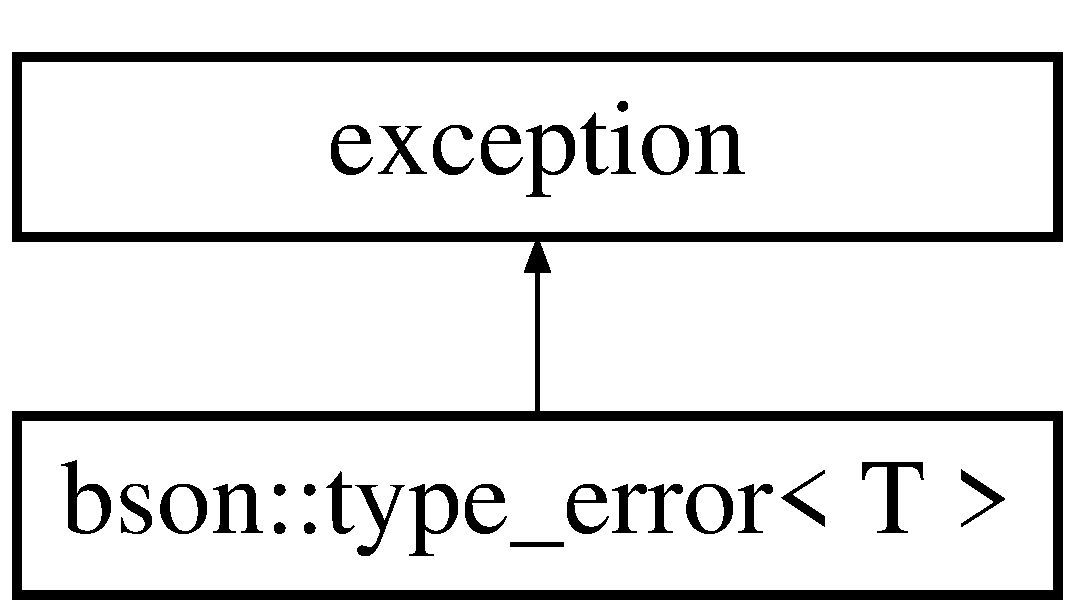
\includegraphics[height=2.000000cm]{classbson_1_1type__error}
\end{center}
\end{figure}
\subsection*{Public Member Functions}
\begin{DoxyCompactItemize}
\item 
\hypertarget{classbson_1_1type__error_a14050384ee0b381c905caa1cf68991ec}{{\bfseries type\+\_\+error} (const Type\+Info \&ti)}\label{classbson_1_1type__error_a14050384ee0b381c905caa1cf68991ec}

\item 
\hypertarget{classbson_1_1type__error_ac7ca3c1cfb5c8ae9865b3385c3e3d327}{virtual const char $\ast$ {\bfseries what} () const noexcept}\label{classbson_1_1type__error_ac7ca3c1cfb5c8ae9865b3385c3e3d327}

\end{DoxyCompactItemize}


The documentation for this class was generated from the following file\+:\begin{DoxyCompactItemize}
\item 
\hyperlink{typeinfo_8h}{typeinfo.\+h}\end{DoxyCompactItemize}

\hypertarget{classbson_1_1type___u_n_k_n_o_w_n}{\section{bson\+:\+:type\+\_\+\+U\+N\+K\+N\+O\+W\+N Class Reference}
\label{classbson_1_1type___u_n_k_n_o_w_n}\index{bson\+::type\+\_\+\+U\+N\+K\+N\+O\+W\+N@{bson\+::type\+\_\+\+U\+N\+K\+N\+O\+W\+N}}
}
Inheritance diagram for bson\+:\+:type\+\_\+\+U\+N\+K\+N\+O\+W\+N\+:\begin{figure}[H]
\begin{center}
\leavevmode
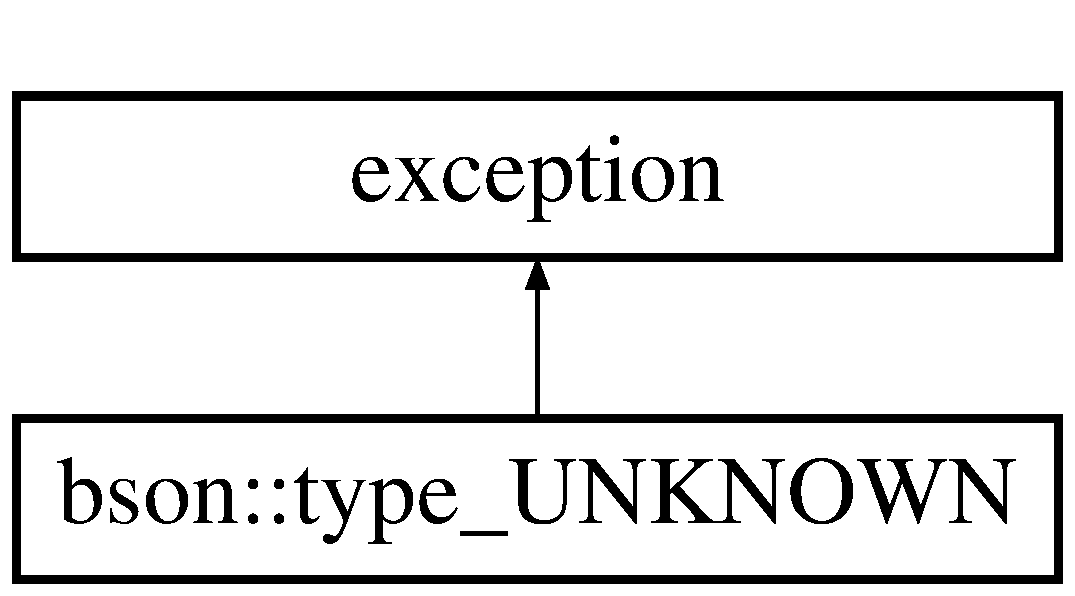
\includegraphics[height=2.000000cm]{classbson_1_1type___u_n_k_n_o_w_n}
\end{center}
\end{figure}
\subsection*{Public Member Functions}
\begin{DoxyCompactItemize}
\item 
\hypertarget{classbson_1_1type___u_n_k_n_o_w_n_ae8217518b2f8354d889b5594cc900751}{virtual const char $\ast$ {\bfseries what} () const noexcept}\label{classbson_1_1type___u_n_k_n_o_w_n_ae8217518b2f8354d889b5594cc900751}

\end{DoxyCompactItemize}


The documentation for this class was generated from the following file\+:\begin{DoxyCompactItemize}
\item 
\hyperlink{typeinfo_8h}{typeinfo.\+h}\end{DoxyCompactItemize}

\chapter{File Documentation}
\hypertarget{document_8h}{\section{document.\+h File Reference}
\label{document_8h}\index{document.\+h@{document.\+h}}
}


Definition of the B\+S\+O\+N Document class.  


{\ttfamily \#include \char`\"{}element.\+h\char`\"{}}\\*
{\ttfamily \#include \char`\"{}typeinfo\char`\"{}}\\*
{\ttfamily \#include $<$initializer\+\_\+list$>$}\\*
{\ttfamily \#include $<$map$>$}\\*
{\ttfamily \#include $<$set$>$}\\*
{\ttfamily \#include $<$sstream$>$}\\*
{\ttfamily \#include $<$ostream$>$}\\*
\subsection*{Classes}
\begin{DoxyCompactItemize}
\item 
class \hyperlink{classbson_1_1_document}{bson\+::\+Document}
\end{DoxyCompactItemize}
\subsection*{Functions}
\begin{DoxyCompactItemize}
\item 
std\+::ostream \& {\bfseries bson\+::operator$<$$<$} (std\+::ostream \&oss, const Document \&d)
\end{DoxyCompactItemize}


\subsection{Detailed Description}
Definition of the B\+S\+O\+N Document class. 

\begin{DoxyAuthor}{Author}
Nathan Eloe 
\end{DoxyAuthor}

\hypertarget{element_8h}{\section{element.\+h File Reference}
\label{element_8h}\index{element.\+h@{element.\+h}}
}


Declaration of a B\+S\+O\+N element.  


{\ttfamily \#include \char`\"{}typeinfo.\+h\char`\"{}}\\*
{\ttfamily \#include $<$sstream$>$}\\*
{\ttfamily \#include $<$memory$>$}\\*
{\ttfamily \#include $<$vector$>$}\\*
{\ttfamily \#include \char`\"{}template\+\_\+spec/document.\+hpp\char`\"{}}\\*
{\ttfamily \#include \char`\"{}template\+\_\+spec/floats.\+hpp\char`\"{}}\\*
{\ttfamily \#include \char`\"{}template\+\_\+spec/strings.\+hpp\char`\"{}}\\*
{\ttfamily \#include \char`\"{}template\+\_\+spec/ints.\+hpp\char`\"{}}\\*
{\ttfamily \#include \char`\"{}template\+\_\+spec/bools.\+hpp\char`\"{}}\\*
{\ttfamily \#include \char`\"{}template\+\_\+spec/vectors.\+hpp\char`\"{}}\\*
{\ttfamily \#include \char`\"{}template\+\_\+spec/chararrs.\+hpp\char`\"{}}\\*
{\ttfamily \#include \char`\"{}template\+\_\+spec/voids.\+hpp\char`\"{}}\\*
{\ttfamily \#include \char`\"{}template\+\_\+spec/pairs.\+hpp\char`\"{}}\\*
{\ttfamily \#include \char`\"{}template\+\_\+spec/jsscope.\+hpp\char`\"{}}\\*
{\ttfamily \#include \char`\"{}template\+\_\+spec/binary.\+hpp\char`\"{}}\\*
{\ttfamily \#include \char`\"{}element.\+hpp\char`\"{}}\\*
\subsection*{Classes}
\begin{DoxyCompactItemize}
\item 
class \hyperlink{classbson_1_1_element}{bson\+::\+Element}
\end{DoxyCompactItemize}
\subsection*{Typedefs}
\begin{DoxyCompactItemize}
\item 
\hypertarget{namespacebson_a889cbd9b6722f0ca0ce7e6e0152dbb08}{typedef std\+::vector$<$ Element $>$ {\bfseries bson\+::array}}\label{namespacebson_a889cbd9b6722f0ca0ce7e6e0152dbb08}

\item 
\hypertarget{namespacebson_a098262b719467d3ccb2b4e7f8a2c405b}{typedef std\+::array$<$ unsigned \\*
char, O\+I\+D\+\_\+\+S\+I\+Z\+E $>$ {\bfseries bson\+::oid}}\label{namespacebson_a098262b719467d3ccb2b4e7f8a2c405b}

\item 
\hypertarget{namespacebson_aa858fc77fdde42053b7654d89fb4aea9}{typedef std\+::pair$<$ std\+::string, \\*
std\+::string $>$ {\bfseries bson\+::regex}}\label{namespacebson_aa858fc77fdde42053b7654d89fb4aea9}

\item 
\hypertarget{namespacebson_a3f3051610a757567afeb6d8df926eb4b}{typedef std\+::pair$<$ std\+::string, \\*
std\+::array$<$ unsigned char, \\*
D\+B\+\_\+\+P\+T\+R\+\_\+\+S\+I\+Z\+E $>$ $>$ {\bfseries bson\+::dbptr}}\label{namespacebson_a3f3051610a757567afeb6d8df926eb4b}

\item 
\hypertarget{namespacebson_ac81ab2cd5826d15fd570d2771f98afd5}{typedef std\+::pair$<$ std\+::string, \\*
Document $>$ {\bfseries bson\+::jscode\+\_\+scope}}\label{namespacebson_ac81ab2cd5826d15fd570d2771f98afd5}

\item 
\hypertarget{namespacebson_a59d8f7e0753d7db58b777995f8f0412d}{typedef std\+::pair$<$ unsigned \\*
char, std\+::string $>$ {\bfseries bson\+::binary}}\label{namespacebson_a59d8f7e0753d7db58b777995f8f0412d}

\end{DoxyCompactItemize}
\subsection*{Functions}
\begin{DoxyCompactItemize}
\item 
{\footnotesize template$<$typename T $>$ }\\std\+::string {\bfseries bson\+::to\+\_\+string} ()
\begin{DoxyCompactList}\small\item\em converts a type name to a string (for exceptions) \end{DoxyCompactList}\item 
{\footnotesize template$<$typename T $>$ }\\Type\+Info {\bfseries bson\+::default\+\_\+type} ()
\begin{DoxyCompactList}\small\item\em determines the default type for type T \end{DoxyCompactList}\end{DoxyCompactItemize}
\subsection*{Variables}
\begin{DoxyCompactItemize}
\item 
\hypertarget{namespacebson_a11c2d5c3578fe201ed59df9ac0e87a79}{const char {\bfseries bson\+::\+X00} = '\textbackslash{}0'}\label{namespacebson_a11c2d5c3578fe201ed59df9ac0e87a79}

\item 
\hypertarget{namespacebson_a7b88049f5cec530b486e5ed1102ca5f0}{const int {\bfseries bson\+::\+O\+I\+D\+\_\+\+S\+I\+Z\+E} = 12}\label{namespacebson_a7b88049f5cec530b486e5ed1102ca5f0}

\item 
\hypertarget{namespacebson_aeed8c1e4d6f43f30283073a6e0a68c69}{const int {\bfseries bson\+::\+D\+B\+\_\+\+P\+T\+R\+\_\+\+S\+I\+Z\+E} = 12}\label{namespacebson_aeed8c1e4d6f43f30283073a6e0a68c69}

\end{DoxyCompactItemize}


\subsection{Detailed Description}
Declaration of a B\+S\+O\+N element. 

\begin{DoxyAuthor}{Author}
Nathan Eloe 
\end{DoxyAuthor}

\hypertarget{element_8hpp}{\section{element.\+hpp File Reference}
\label{element_8hpp}\index{element.\+hpp@{element.\+hpp}}
}


Implementation of the B\+S\+O\+N element class.  


{\ttfamily \#include \char`\"{}element.\+h\char`\"{}}\\*
{\ttfamily \#include \char`\"{}typeinfo.\+h\char`\"{}}\\*
{\ttfamily \#include $<$memory$>$}\\*
{\ttfamily \#include $<$vector$>$}\\*


\subsection{Detailed Description}
Implementation of the B\+S\+O\+N element class. 

\begin{DoxyAuthor}{Author}
Nathan Eloe 
\end{DoxyAuthor}

\hypertarget{typeinfo_8h}{\section{typeinfo.\+h File Reference}
\label{typeinfo_8h}\index{typeinfo.\+h@{typeinfo.\+h}}
}


Enumeration to keep track of types for bson.  


{\ttfamily \#include $<$exception$>$}\\*
{\ttfamily \#include $<$string$>$}\\*
{\ttfamily \#include $<$boost/concept\+\_\+check.\+hpp$>$}\\*
\subsection*{Classes}
\begin{DoxyCompactItemize}
\item 
class \hyperlink{classbson_1_1type__error}{bson\+::type\+\_\+error$<$ T $>$}
\item 
class \hyperlink{classbson_1_1type___u_n_k_n_o_w_n}{bson\+::type\+\_\+\+U\+N\+K\+N\+O\+W\+N}
\end{DoxyCompactItemize}
\subsection*{Enumerations}
\begin{DoxyCompactItemize}
\item 
\hypertarget{namespacebson_a6c41ff65d733f64ff5eb13a94452a063}{enum {\bfseries Type\+Info} \{ \\*
{\bfseries \+\_\+\+U\+N\+K\+N\+O\+W\+N} =0, 
{\bfseries F\+L\+O\+A\+T\+I\+N\+G} =1, 
{\bfseries S\+T\+R\+I\+N\+G}, 
{\bfseries D\+O\+C\+U\+M\+E\+N\+T}, 
\\*
{\bfseries A\+R\+R\+A\+Y}, 
{\bfseries B\+I\+N\+A\+R\+Y}, 
{\bfseries U\+N\+D\+E\+F}, 
{\bfseries O\+I\+D}, 
\\*
{\bfseries B\+O\+O\+L}, 
{\bfseries D\+A\+T\+E\+T\+I\+M\+E}, 
{\bfseries N\+I\+L}, 
{\bfseries R\+E\+G\+E\+X}, 
\\*
{\bfseries D\+B\+P\+T\+R}, 
{\bfseries J\+S}, 
{\bfseries D\+E\+P\+R\+E\+C\+A\+T\+E\+D}, 
{\bfseries J\+S\+\_\+\+S\+C\+O\+P\+E}, 
\\*
{\bfseries I\+N\+T32}, 
{\bfseries T\+I\+M\+E\+S\+T\+A\+M\+P}, 
{\bfseries I\+N\+T64}, 
{\bfseries M\+I\+N\+K\+E\+Y} =0x\+F\+F, 
\\*
{\bfseries M\+A\+X\+K\+E\+Y} =0x7\+F
 \}}\label{namespacebson_a6c41ff65d733f64ff5eb13a94452a063}

\end{DoxyCompactItemize}
\subsection*{Functions}
\begin{DoxyCompactItemize}
\item 
\hypertarget{namespacebson_a77b2d6189553c48d5c56c6b6431ea5b6}{char {\bfseries bson\+::to\+\_\+char} (const Type\+Info \&ti)}\label{namespacebson_a77b2d6189553c48d5c56c6b6431ea5b6}

\item 
{\footnotesize template$<$typename T $>$ }\\std\+::string {\bfseries bson\+::to\+\_\+string} ()
\begin{DoxyCompactList}\small\item\em converts a type name to a string (for exceptions) \end{DoxyCompactList}\item 
\hypertarget{namespacebson_a8abf70aa907f60b3f25d71cdb02e679d}{std\+::string {\bfseries bson\+::to\+\_\+string} (const Type\+Info \&ti)}\label{namespacebson_a8abf70aa907f60b3f25d71cdb02e679d}

\end{DoxyCompactItemize}
\subsection*{Variables}
\begin{DoxyCompactItemize}
\item 
const std\+::string {\bfseries bson\+::\+N\+A\+M\+E\+S} \mbox{[}$\,$\mbox{]}
\end{DoxyCompactItemize}


\subsection{Detailed Description}
Enumeration to keep track of types for bson. 

\begin{DoxyAuthor}{Author}
Nathan Eloe 
\end{DoxyAuthor}

%--- End generated contents ---

% Index
\newpage
\phantomsection
\addcontentsline{toc}{chapter}{Index}
\printindex

\end{document}
